\\ \hrule \smallskip 
\textbf{Question 47.} \\
\hrule 

Return to the credit card scenario of Exercise 12 (Section 2.2), and let $C$ be the event that the selected student has an American Express card. In addition to $P(A) = .6$, $P(B) = .4$, and $P(A \cap B) = .3$, suppose that $P(C) = .2$, $P(A \cap C) = .15$, $P(B \cap C)$, and $P(A \cap B \cap C) = .08$.

Before we get started, let's make a Venn diagram that we can utilize. I would explain where the smaller intersections came from better, but I'm running out of time to transcribe these notes! Simply put, I took the given intersections and removed the triple intersection to get the values. 

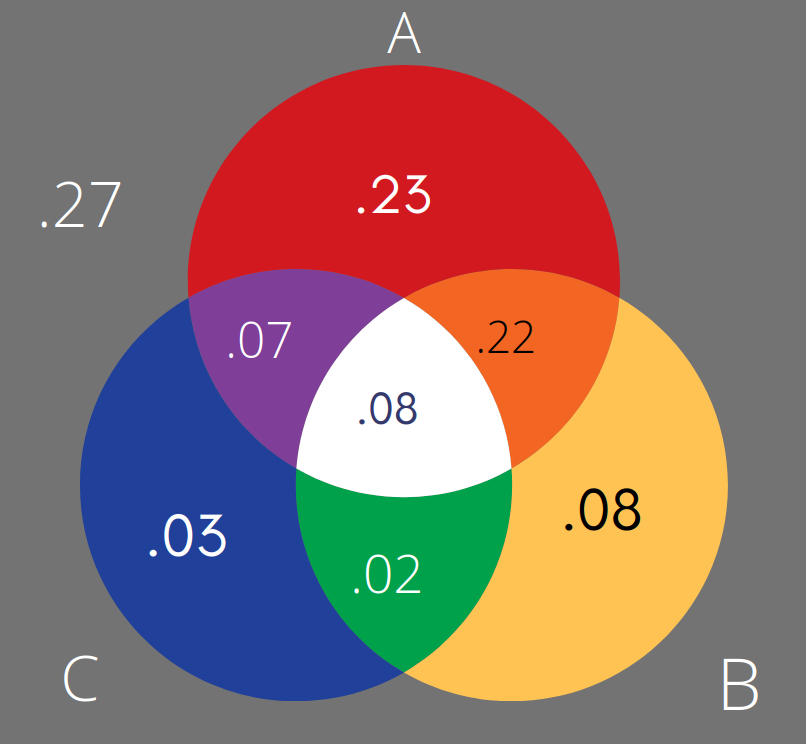
\includegraphics[scale=.25]{images/whw3/2.4.47_venn.png}

\textbf{a. What is the probability that the selected student has at least one of the three types of cards?} \newline 
$P(A \cup B \cup C)$ is the inside of the venn diagram all added together, what we get from this is $\boxed{= 0.74}$

\textbf{b. What is the probability that the selected student has both a Visa card and a Mastercard but not an American Express card?} \newline
$P(A \cap B \cap C')$ is what we're solving for here. Using the venn diagram, we know this is part of our intersections and it's our one intersection that doesn't involve C. So, we get $\boxed{.22}$. 

\textbf{c. Calculate and interpret $P(B|A)$ and also $P(A|B)$.}
\[P(B|A) = \frac{P(B \cap A)}{P(A)} = \frac{0.3}{0.6} = \boxed{.5}\]
\[P(A|B) = \frac{P(A \cap B)}{P(B)} = \frac{0.3}{0.4} = \boxed{.75}\]

What we can say from these two calculations is that if a student has a Visa card, there is a 50\% chance that they also have a MasterCard. We can also say that if a student has a MasterCard, there is a 75\% chance that they have a Visa. 

\textbf{d. If we learn that the selected student has an American Express card, what is the probability that she or he also has both a Visa card and a MasterCard?}
\[P(A \cap B | C) = \frac{P(A \cap B \cap C)}{P(C)} = \frac{.08}{.2} = \boxed{.4}\]

\textbf{e. Given that the selected student has an American Express card, what is the probability that she or he has at least one of the other two types of cards?}
\[P(A \cup B|C) = \frac{P((A \cup B) \cap C)}{P(C)} = \frac{.07+.08+.02}{.2} = \boxed{.85}\]